\documentclass[10pt,fleqn]{article} % Default font size and left-justified equations
\usepackage[%
    pdftitle={Informatique : capteur rayonnement},
    pdfauthor={Xavier Pessoles}]{hyperref}

%%%%%%%%%%%%%%%%%%%%%%%%%%%%%%%%%%%%%%%%%
% Original author:
% Mathias Legrand (legrand.mathias@gmail.com) with modifications by:
% Vel (vel@latextemplates.com)
% License:
% CC BY-NC-SA 3.0 (http://creativecommons.org/licenses/by-nc-sa/3.0/)
%%%%%%%%%%%%%%%%%%%%%%%%%%%%%%%%%%%%%%%%%

%----------------------------------------------------------------------------------------
%	VARIOUS REQUIRED PACKAGES AND CONFIGURATIONS
%----------------------------------------------------------------------------------------

\usepackage[top=2.5cm,bottom=2cm,left=2cm,right=2cm,headsep=40pt,a4paper]{geometry} % Page margins

\usepackage{graphicx} % Required for including pictures
\graphicspath{{images/}} % Specifies the directory where pictures are stored

\usepackage{lipsum} % Inserts dummy text

\usepackage{tikz} % Required for drawing custom shapes

\usepackage[french]{babel} % English language/hyphenation
\frenchbsetup{StandardLists=true} % Pour éviter la collision babel enumitem pour les listes

\usepackage{enumitem} % Customize lists
\setlist{nolistsep} % Reduce spacing between bullet points and numbered lists

\usepackage{booktabs} % Required for nicer horizontal rules in tables

\usepackage{xcolor} % Required for specifying colors by name
%\definecolor{ocre}{RGB}{243,102,25} % Define the orange color used for highlighting throughout the book
 \definecolor{ocre}{RGB}{49,133,156} % Couleur ''bleue''
\definecolor{violetf}{RGB}{112,48,160} % Couleur ''violet''
\usepackage{enumitem}
\usepackage{pifont} % Pour les dinglist
\usepackage{multicol}
\usepackage{array} % Centrage vertical dans les tableaux

%----------------------------------------------------------------------------------------
%	FONTS
%----------------------------------------------------------------------------------------

\usepackage{avant} % Use the Avantgarde font for headings
%\usepackage{times} % Use the Times font for headings
%\usepackage{mathptmx} % Use the Adobe Times Roman as the default text font together with math symbols from the Sym­bol, Chancery and Com­puter Modern fonts
\usepackage[adobe-utopia]{mathdesign}
\usepackage{microtype} % Slightly tweak font spacing for aesthetics
\usepackage[utf8]{inputenc} % Required for including letters with accents
\usepackage[T1]{fontenc} % Use 8-bit encoding that has 256 glyphs

%----------------------------------------------------------------------------------------
%	BIBLIOGRAPHY AND INDEX
%----------------------------------------------------------------------------------------

\usepackage[style=alphabetic,citestyle=numeric,sorting=nyt,sortcites=true,autopunct=true,babel=hyphen,hyperref=true,abbreviate=false,backref=true,backend=biber]{biblatex}
\addbibresource{bibliography.bib} % BibTeX bibliography file
\defbibheading{bibempty}{}

\usepackage{calc} % For simpler calculation - used for spacing the index letter headings correctly
\usepackage{makeidx} % Required to make an index
\makeindex % Tells LaTeX to create the files required for indexing

%----------------------------------------------------------------------------------------
%	MAIN TABLE OF CONTENTS
%----------------------------------------------------------------------------------------

\usepackage{titletoc} % Required for manipulating the table of contents

\setcounter{tocdepth}{2}     % Dans la table des matieres
\setcounter{secnumdepth}{2}

\contentsmargin{0cm} % Removes the default margin

% Part text styling
\titlecontents{part}[0cm]
{\addvspace{20pt}\centering\large\bfseries}
{}
{}
{}

% Chapter text styling
\titlecontents{chapter}[1.25cm] % Indentation
{\addvspace{12pt}\large\sffamily\bfseries} % Spacing and font options for chapters
{\color{ocre!60}\contentslabel[\Large\thecontentslabel]{1.25cm}\color{ocre}} % Chapter number
{\color{ocre}}  
{\color{ocre!60}\normalsize\;\titlerule*[.5pc]{.}\;\thecontentspage} % Page number

% Section text styling
\titlecontents{section}[1.25cm] % Indentation
{\addvspace{3pt}\sffamily\bfseries} % Spacing and font options for sections
{\color{ocre!60}\contentslabel[\thecontentslabel]{1.25cm} \color{ocre}} % Section number
{\color{ocre}}
{\hfill\color{ocre!60}\thecontentspage} % Page number
[]

% Subsection text styling
\titlecontents{subsection}[1.25cm] % Indentation
{\addvspace{1pt}\sffamily\small} % Spacing and font options for subsections
{\contentslabel[\thecontentslabel]{1.25cm}} % Subsection number
{}
{\ \titlerule*[.5pc]{.}\;\thecontentspage} % Page number
[]

% List of figures
\titlecontents{figure}[0em]
{\addvspace{-5pt}\sffamily}
{\thecontentslabel\hspace*{1em}}
{}
{\ \titlerule*[.5pc]{.}\;\thecontentspage}
[]

% List of tables
\titlecontents{table}[0em]
{\addvspace{-5pt}\sffamily}
{\thecontentslabel\hspace*{1em}}
{}
{\ \titlerule*[.5pc]{.}\;\thecontentspage}
[]

%----------------------------------------------------------------------------------------
%	MINI TABLE OF CONTENTS IN PART HEADS
%----------------------------------------------------------------------------------------

% Chapter text styling
\titlecontents{lchapter}[0em] % Indenting
{\addvspace{15pt}\large\sffamily\bfseries} % Spacing and font options for chapters
{\color{ocre}\contentslabel[\Large\thecontentslabel]{1.25cm}\color{ocre}} % Chapter number
{}  
{\color{ocre}\normalsize\sffamily\bfseries\;\titlerule*[.5pc]{.}\;\thecontentspage} % Page number

% Section text styling
\titlecontents{lsection}[0em] % Indenting
{\sffamily\small} % Spacing and font options for sections
{\contentslabel[\thecontentslabel]{1.25cm}} % Section number
{}
{}

% Subsection text styling
\titlecontents{lsubsection}[.5em] % Indentation
{\normalfont\footnotesize\sffamily} % Font settings
{}
{}
{}

%----------------------------------------------------------------------------------------
%	PAGE HEADERS
%----------------------------------------------------------------------------------------

\usepackage{fancyhdr} % Required for header and footer configuration



\pagestyle{fancy}
 \renewcommand{\headrulewidth}{0pt}
 \fancyhead{}
 \fancyhead[L]{%
 \noindent\begin{minipage}[c]{2.6cm}%
 
\includegraphics[width=2cm]{png/logo_lycee.png}%
 \end{minipage}}

\fancyhead[C]{\rule{8cm}{.5pt}}

 \fancyhead[R]{%
 \noindent\begin{minipage}[c]{3cm}
 \begin{flushright}
 \footnotesize{\textit{\textsf{\xxtete}}}%
 \end{flushright}
 \end{minipage}
}


\fancyfoot[C]{\rule{12cm}{.5pt}}
\renewcommand{\footrulewidth}{0.2pt}
\fancyfoot[C]{\footnotesize{\bfseries \thepage}}
\fancyfoot[L]{ 
\begin{minipage}[c]{.2\linewidth}
\noindent\footnotesize{{\xxauteur}}
\end{minipage}}


\fancyfoot[R]{\footnotesize{\xxpied}
\ifthenelse{\isodd{\value{page}}}{
\begin{tikzpicture}[overlay]
\node[shape=rectangle, 
      rounded corners = .25 cm,
	  draw= ocre,
	  line width=2pt, 
	  fill = ocre!10,
	  minimum width  = 2.5cm,
	  minimum height = 3cm,] at (\xxposongletx,\xxposonglety) {};
\node at (\xxposonglettext,\xxposonglety) {\rotatebox{90}{\textbf{\large\color{ocre}{\xxonglet}}}};
%{};
\end{tikzpicture}}{}
}
%
%
%
% Removes the header from odd empty pages at the end of chapters
\makeatletter
\renewcommand{\cleardoublepage}{
\clearpage\ifodd\c@page\else
\hbox{}
\vspace*{\fill}
\thispagestyle{empty}
\newpage
\fi}

\fancypagestyle{plain}{%
\fancyhf{} % vide l’en-tête et le pied~de~page.
%\fancyfoot[C]{\bfseries \thepage} % numéro de la page en cours en gras
% et centré en pied~de~page.
\fancyfoot[R]{\footnotesize{\xxpied}}
\fancyfoot[C]{\rule{12cm}{.5pt}}
\renewcommand{\footrulewidth}{0.2pt}
\fancyfoot[C]{\footnotesize{\bfseries \thepage}}
\fancyfoot[L]{ 
\begin{minipage}[c]{.2\linewidth}
\noindent\footnotesize{{\xxauteur}}
\end{minipage}}}



%----------------------------------------------------------------------------------------
%	THEOREM STYLES
%----------------------------------------------------------------------------------------

% Conflit avec la police adobe
%\usepackage{amsmath,amsfonts,amssymb,amsthm} % For math equations, theorems, symbols, etc
\usepackage{amsmath,amsthm}

\newcommand{\intoo}[2]{\mathopen{]}#1\,;#2\mathclose{[}}
\newcommand{\ud}{\mathop{\mathrm{{}d}}\mathopen{}}
\newcommand{\intff}[2]{\mathopen{[}#1\,;#2\mathclose{]}}
%\newtheorem{notation}{Notation}[chapter]
\newtheorem{notation}{Notation}[section]

% Boxed/framed environments
\newtheoremstyle{ocrenumbox}% % Theorem style name
{0pt}% Space above
{0pt}% Space below
{\normalfont}% % Body font
{}% Indent amount
{\small\bf\sffamily\color{ocre}}% % Theorem head font
{\;}% Punctuation after theorem head
{0.25em}% Space after theorem head
{\small\sffamily\color{ocre}\thmname{#1}\nobreakspace\thmnumber%{\@ifnotempty{#1}{}\@upn{#2}}% Theorem text (e.g. Theorem 2.1)
\thmnote{\nobreakspace\the\thm@notefont\sffamily\bfseries\color{black}---\nobreakspace#3.}} % Optional theorem note
\renewcommand{\qedsymbol}{$\blacksquare$}% Optional qed square


% Boite pour les corriges
\newtheoremstyle{correctionbox}% % Theorem style name
{0pt}% Space above
{0pt}% Space below
{\normalfont}% % Body font
{}% Indent amount
{\small\bf\sffamily\color{violet}}% % Theorem head font
{\;}% Punctuation after theorem head
{0.25em}% Space after theorem head
{\small\sffamily\color{ocre}\thmname{#1}\nobreakspace\thmnumber%{\@ifnotempty{#1}{}\@upn{#2}}% Theorem text (e.g. Theorem 2.1)
\thmnote{\nobreakspace\the\thm@notefont\sffamily\bfseries\color{black}---\nobreakspace#3.}} % Optional theorem note
\renewcommand{\qedsymbol}{$\blacksquare$}% Optional qed square



\newtheoremstyle{blacknumex}% Theorem style name
{5pt}% Space above
{5pt}% Space below
{\normalfont}% Body font
{} % Indent amount
{\small\bf\sffamily}% Theorem head font
{\;}% Punctuation after theorem head
{0.25em}% Space after theorem head
{\small\sffamily{\tiny\ensuremath{\blacksquare}}\nobreakspace\thmname{#1}\nobreakspace\thmnumber%{\@ifnotempty{#1}{}\@upn{#2}}% Theorem text (e.g. Theorem 2.1)
\thmnote{\nobreakspace\the\thm@notefont\sffamily\bfseries---\nobreakspace#3.}}% Optional theorem note

\newtheoremstyle{blacknumbox} % Theorem style name
{0pt}% Space above
{0pt}% Space below
{\normalfont}% Body font
{}% Indent amount
{\small\bf\sffamily}% Theorem head font
{\;}% Punctuation after theorem head
{0.25em}% Space after theorem head
{\small\sffamily\thmname{#1}\nobreakspace 
\thmnote{\nobreakspace\the\thm@notefont\sffamily\bfseries---\nobreakspace#3.}}% Optional theorem note

% Non-boxed/non-framed environments
\newtheoremstyle{ocrenum}% % Theorem style name
{5pt}% Space above
{5pt}% Space below
{\normalfont}% % Body font
{}% Indent amount
{\small\bf\sffamily\color{ocre}}% % Theorem head font
{\;}% Punctuation after theorem head
{0.25em}% Space after theorem head
{\small\sffamily\color{ocre}\thmname{#1}\nobreakspace\thmnumber{\@ifnotempty{#1}{}\@upn{#2}}% Theorem text (e.g. Theorem 2.1)
\thmnote{\nobreakspace\the\thm@notefont\sffamily\bfseries\color{black}---\nobreakspace#3.}} % Optional theorem note
\renewcommand{\qedsymbol}{$\blacksquare$}% Optional qed square
\makeatother

% Environnement pour les titres de parties
\newtheoremstyle{partiebox} 
{0pt}% Space above
{0pt}% Space below
{\normalfont}% Body font
{}% Indent amount
{\small\bf\sffamily}% Theorem head font
{\;}% Punctuation after theorem head
{0.25em}% Space after theorem head




% Defines the theorem text style for each type of theorem to one of the three styles above
\newcounter{dummy} 
\numberwithin{dummy}{section}
\theoremstyle{ocrenumbox}
%\newtheorem{theoremeT}[dummy]{Théorème}
\newtheorem{theoremeT}[dummy]{Théorème}
\newtheorem{resultatT}[dummy]{Résultat}
\newtheorem{savoirT}[dummy]{Savoir}
\newtheorem{methodeT}[dummy]{Méthode}
\newtheorem{objectifT}[dummy]{Objectif}
%\newtheorem{problem}{Problem}[chapter]
\newtheorem{problem}{Problem}[section]
%\newtheorem{exerciseT}{Exercise}[chapter]
\newtheorem{exerciseT}{Exercice}[section]

\theoremstyle{blacknumex}
%\newtheorem{exampleT}{Example}[chapter]
\newtheorem{exempleT}{Exemple}[section]
\newtheorem{termT}{Terminal\\}[section]
\newtheorem{pyT}{Python\\}[section]
\newtheorem{sciT}{Scilab\\}[section]

\theoremstyle{blacknumbox}
%\newtheorem{vocabulary}{Vocabulary}[chapter]
\newtheorem{vocabulary}{Vocabulaire}[section]
%\newtheorem{definitionT}{Definition}[section]
\newtheorem{definitionT}{Définition}[section]
\newtheorem{demoT}{Démonstration}[section]
\newtheorem{corollaryT}[dummy]{Corollaire}
\newtheorem{hypoT}{Hypothèse(s)}

\theoremstyle{ocrenum}
\newtheorem{proposition}[dummy]{Proposition}

\theoremstyle{partiebox}
\newtheorem{titrepartieT}[]{}
\newtheorem{titrechapitreT}[]{}

\theoremstyle{correctionbox}
\newtheorem{correctionT}[dummy]{\color{violet}{Correction}}

%----------------------------------------------------------------------------------------
%	DEFINITION OF COLORED BOXES
%----------------------------------------------------------------------------------------

\RequirePackage[framemethod=tikz]{mdframed} % Required for creating the theorem, definition, exercise and corollary boxes

% Theorem box
\newmdenv[skipabove=7pt,
skipbelow=7pt,
backgroundcolor=ocre!10,
linecolor=ocre,
innerleftmargin=5pt,
innerrightmargin=5pt,
innertopmargin=5pt,
leftmargin=0cm,
rightmargin=0cm,
innerbottommargin=5pt]{tBox}


% Correction
\newmdenv[skipabove=7pt,
skipbelow=7pt,
backgroundcolor=violet!10,
linecolor=violet,
innerleftmargin=5pt,
innerrightmargin=5pt,
innertopmargin=5pt,
leftmargin=0cm,
rightmargin=0cm,
innerbottommargin=5pt]{coBox}


% Exercise box	  
\newmdenv[skipabove=7pt,
skipbelow=7pt,
rightline=false,
leftline=true,
topline=false,
bottomline=false,
backgroundcolor=ocre!10,
linecolor=ocre,
innerleftmargin=5pt,
innerrightmargin=5pt,
innertopmargin=5pt,
innerbottommargin=5pt,
leftmargin=0cm,
rightmargin=0cm,
linewidth=4pt]{eBox}	

% Definition box
\newmdenv[skipabove=7pt,
skipbelow=7pt,
rightline=false,
leftline=true,
topline=false,
bottomline=false,
backgroundcolor=ocre!10,
linecolor=ocre,
innerleftmargin=5pt,
innerrightmargin=5pt,
innertopmargin=0pt,
leftmargin=0cm,
rightmargin=0cm,
linewidth=4pt,
innerbottommargin=0pt]{dBox}	

% Demonstration box
\newmdenv[skipabove=7pt,
skipbelow=7pt,
rightline=false,
leftline=true,
topline=false,
bottomline=false,
%backgroundcolor=ocre!10,
linecolor=ocre,
innerleftmargin=5pt,
innerrightmargin=5pt,
innertopmargin=0pt,
leftmargin=0cm,
rightmargin=0cm,
linewidth=4pt,
innerbottommargin=0pt]{demoBox}	

% Corollary box
\newmdenv[skipabove=7pt,
skipbelow=7pt,
rightline=false,
leftline=true,
topline=false,
bottomline=false,
linecolor=gray,
backgroundcolor=black!5,
innerleftmargin=5pt,
innerrightmargin=5pt,
innertopmargin=5pt,
leftmargin=0cm,
rightmargin=0cm,
linewidth=4pt,
innerbottommargin=5pt]{cBox}


% Hypothèses
\newmdenv[skipabove=7pt,
skipbelow=7pt,
rightline=false,
leftline=true,
topline=false,
bottomline=false,
linecolor=gray,
backgroundcolor=black!5,
innerleftmargin=5pt,
innerrightmargin=5pt,
innertopmargin=5pt,
leftmargin=0cm,
rightmargin=0cm,
linewidth=4pt,
innerbottommargin=5pt]{hyBox}


% Boite pour le titre de la partie (pBox)
\newmdenv[skipabove=7pt,
skipbelow=7pt,
rightline=true,
leftline=false,
topline=false,
bottomline=false,
linecolor=ocre,
backgroundcolor=none,
innerleftmargin=5pt,
innerrightmargin=5pt,
innertopmargin=5pt,
leftmargin=0cm,
rightmargin=0cm,
linewidth=4pt,
innerbottommargin=5pt]{pBox}

% Boite pour le titre du chapitre (chBox)
\newmdenv[skipabove=7pt,
skipbelow=7pt,
rightline=false,
leftline=true,
topline=false,
bottomline=false,
linecolor=ocre,
%backgroundcolor=black!5,
innerleftmargin=5pt,
innerrightmargin=5pt,
innertopmargin=5pt,
leftmargin=0cm,
rightmargin=0cm,
linewidth=4pt,
innerbottommargin=5pt]{chBox}


% Boite pour les exemples
\newmdenv[skipabove=7pt,
skipbelow=7pt,
rightline=false,
leftline=true,
topline=false,
bottomline=false,
linecolor=gray,
backgroundcolor=white,
innerleftmargin=5pt,
innerrightmargin=5pt,
innertopmargin=5pt,
leftmargin=0cm,
rightmargin=0cm,
linewidth=4pt,
innerbottommargin=5pt]{exBox}

% Boite pour le terminal
\newmdenv[skipabove=7pt,
skipbelow=7pt,
rightline=false,
leftline=true,
topline=false,
bottomline=false,
linecolor=gray,
backgroundcolor=white,
innerleftmargin=5pt,
innerrightmargin=5pt,
innertopmargin=5pt,
leftmargin=0cm,
rightmargin=0cm,
linewidth=4pt,
innerbottommargin=5pt]{termBox}


% Boite pour Python
\newmdenv[skipabove=7pt,
skipbelow=7pt,
rightline=false,
leftline=true,
topline=false,
bottomline=false,
linecolor=gray,
backgroundcolor=white,
innerleftmargin=5pt,
innerrightmargin=5pt,
innertopmargin=5pt,
leftmargin=0cm,
rightmargin=0cm,
linewidth=4pt,
innerbottommargin=5pt]{pyBox}

% Boite pour scilab
\newmdenv[skipabove=7pt,
skipbelow=7pt,
rightline=false,
leftline=true,
topline=false,
bottomline=false,
linecolor=gray,
backgroundcolor=white,
innerleftmargin=5pt,
innerrightmargin=5pt,
innertopmargin=5pt,
leftmargin=0cm,
rightmargin=0cm,
linewidth=4pt,
innerbottommargin=5pt]{sciBox}
% Creates an environment for each type of theorem and assigns it a theorem text style from the "Theorem Styles" section above and a colored box from above
\newenvironment{theorem}{\begin{tBox}\begin{theoremeT}}{\end{theoremeT}\end{tBox}}
\newenvironment{resultat}{\begin{tBox}\begin{resultatT}}{\end{resultatT}\end{tBox}}
\newenvironment{methode}{\begin{tBox}\begin{methodeT}}{\end{methodeT}\end{tBox}}
\newenvironment{savoir}{\begin{tBox}\begin{savoirT}}{\end{savoirT}\end{tBox}}
\newenvironment{obj}{\begin{tBox}\begin{objectifT}}{\end{objectifT}\end{tBox}}
\newenvironment{corrige}{\begin{coBox}\begin{correctionT}}{\end{correctionT}\end{coBox}}
\newenvironment{exercise}{\begin{eBox}\begin{exerciseT}}{\hfill{\color{ocre}\tiny\ensuremath{\blacksquare}}\end{exerciseT}\end{eBox}}				  
\newenvironment{exercice}{\begin{eBox}\begin{exerciseT}}{\hfill{\color{ocre}\tiny\ensuremath{\blacksquare}}\end{exerciseT}\end{eBox}}				  

\newenvironment{definition}{\begin{dBox}\begin{definitionT}}{\end{definitionT}\end{dBox}}	
\newenvironment{defi}{\begin{dBox}\begin{definitionT}}{\end{definitionT}\end{dBox}}	
\newenvironment{demo}{\begin{demoBox}\begin{demoT}}{\end{demoT}\end{demoBox}}	
%\newenvironment{exemple}{\begin{exempleT}}{\hfill{\tiny\ensuremath{\blacksquare}}\end{exempleT}}		
\newenvironment{corollary}{\begin{cBox}\begin{corollaryT}}{\end{corollaryT}\end{cBox}}
\newenvironment{hypo}{\begin{hyBox}\begin{hypoT}}{\end{hypoT}\end{hyBox}}	\newenvironment{exemple}{\begin{exBox}\begin{exempleT}}{\hfill{\tiny\ensuremath{\blacksquare}}\end{exempleT}\end{exBox}}	
\newenvironment{titrepartie}{\begin{pBox}\begin{titrepartieT}}{\end{titrepartieT}\end{pBox}}	
\newenvironment{titrechapitre}{\begin{chBox}\begin{titrechapitreT}}{\end{titrechapitreT}\end{chBox}}	

\newenvironment{term}{ \begin{termBox}\begin{termT}}{\end{termT}\end{termBox}}
\newenvironment{py}{ \begin{pyBox}\begin{pyT}}{\end{pyT}\end{pyBox}}
\newenvironment{sci}{ \begin{sciBox}\begin{sciT}}{\end{sciT}\end{sciBox}}

%----------------------------------------------------------------------------------------
%	REMARK ENVIRONMENT
%----------------------------------------------------------------------------------------

\newenvironment{remark}{\par\vspace{10pt}\small % Vertical white space above the remark and smaller font size
\begin{list}{}{
\leftmargin=35pt % Indentation on the left
\rightmargin=25pt}\item\ignorespaces % Indentation on the right
\makebox[-2.5pt]{\begin{tikzpicture}[overlay]
\node[draw=ocre!60,line width=1pt,circle,fill=ocre!25,font=\sffamily\bfseries,inner sep=2pt,outer sep=0pt] at (-15pt,0pt){\textcolor{ocre}{R}};\end{tikzpicture}} % Orange R in a circle
\advance\baselineskip -1pt}{\end{list}\vskip5pt} % Tighter line spacing and white space after remark

\newenvironment{rem}{\par\vspace{10pt}\small % Vertical white space above the remark and smaller font size
\begin{list}{}{
\leftmargin=35pt % Indentation on the left
\rightmargin=25pt}\item\ignorespaces % Indentation on the right
\makebox[-2.5pt]{\begin{tikzpicture}[overlay]
\node[draw=ocre!60,line width=1pt,circle,fill=ocre!25,font=\sffamily\bfseries,inner sep=2pt,outer sep=0pt] at (-15pt,0pt){\textcolor{ocre}{R}};\end{tikzpicture}} % Orange R in a circle
\advance\baselineskip -1pt}{\end{list}\vskip5pt} % Tighter line spacing and white space after remark


\newenvironment{warn}{\par\vspace{10pt}\small % Vertical white space above the remark and smaller font size
\begin{list}{}{
\leftmargin=35pt % Indentation on the left
\rightmargin=25pt}\item\ignorespaces % Indentation on the right
\makebox[-2.5pt]{\begin{tikzpicture}[overlay]
\node[draw=red!60,line width=1pt,circle,fill=red!25,font=\sffamily\bfseries,inner sep=2pt,outer sep=0pt] at (-15pt,0pt){\textcolor{black}{!}};\end{tikzpicture}} % Point d'exclamation dans un cercle
\advance\baselineskip -1pt}{\end{list}\vskip5pt} % Tighter line spacing and white space after remark


%----------------------------------------------------------------------------------------
%	SECTION NUMBERING IN THE MARGIN
%----------------------------------------------------------------------------------------

\makeatletter
\renewcommand{\@seccntformat}[1]{\llap{\textcolor{ocre}{\csname the#1\endcsname}\hspace{1em}}}                    
\renewcommand{\section}{\@startsection{section}{1}{\z@}
{-4ex \@plus -1ex \@minus -.4ex}
{1ex \@plus.2ex }
{\normalfont\large\sffamily\bfseries}}
\renewcommand{\subsection}{\@startsection {subsection}{2}{\z@}
{-3ex \@plus -0.1ex \@minus -.4ex}
{0.5ex \@plus.2ex }
{\normalfont\sffamily\bfseries}}
\renewcommand{\subsubsection}{\@startsection {subsubsection}{3}{\z@}
{-2ex \@plus -0.1ex \@minus -.2ex}
{.2ex \@plus.2ex }
{\normalfont\small\sffamily\bfseries}}                        
\renewcommand\paragraph{\@startsection{paragraph}{4}{\z@}
{-2ex \@plus-.2ex \@minus .2ex}
{.1ex}
{\normalfont\small\sffamily\bfseries}}

%----------------------------------------------------------------------------------------
%	PART HEADINGS
%----------------------------------------------------------------------------------------


%----------------------------------------------------------------------------------------
%	CHAPTER HEADINGS
%----------------------------------------------------------------------------------------

% \newcommand{\thechapterimage}{}%
% \newcommand{\chapterimage}[1]{\renewcommand{\thechapterimage}{#1}}%
% \def\@makechapterhead#1{%
% {\parindent \z@ \raggedright \normalfont
% \ifnum \c@secnumdepth >\m@ne
% \if@mainmatter
% \begin{tikzpicture}[remember picture,overlay]
% \node at (current page.north west)
% {\begin{tikzpicture}[remember picture,overlay]
% \node[anchor=north west,inner sep=0pt] at (0,0) {\includegraphics[width=\paperwidth]{\thechapterimage}};
% \draw[anchor=west] (\Gm@lmargin,-9cm) node [line width=2pt,rounded corners=15pt,draw=ocre,fill=white,fill opacity=0.5,inner sep=15pt]{\strut\makebox[22cm]{}};
% \draw[anchor=west] (\Gm@lmargin+.3cm,-9cm) node {\huge\sffamily\bfseries\color{black}\thechapter. #1\strut};
% \end{tikzpicture}};
% \end{tikzpicture}
% \else
% \begin{tikzpicture}[remember picture,overlay]
% \node at (current page.north west)
% {\begin{tikzpicture}[remember picture,overlay]
% \node[anchor=north west,inner sep=0pt] at (0,0) {\includegraphics[width=\paperwidth]{\thechapterimage}};
% \draw[anchor=west] (\Gm@lmargin,-9cm) node [line width=2pt,rounded corners=15pt,draw=ocre,fill=white,fill opacity=0.5,inner sep=15pt]{\strut\makebox[22cm]{}};
% \draw[anchor=west] (\Gm@lmargin+.3cm,-9cm) node {\huge\sffamily\bfseries\color{black}#1\strut};
% \end{tikzpicture}};
% \end{tikzpicture}
% \fi\fi\par\vspace*{270\p@}}}

%-------------------------------------------

\def\@makeschapterhead#1{%
\begin{tikzpicture}[remember picture,overlay]
\node at (current page.north west)
{\begin{tikzpicture}[remember picture,overlay]
\node[anchor=north west,inner sep=0pt] at (0,0) {\includegraphics[width=\paperwidth]{\thechapterimage}};
\draw[anchor=west] (\Gm@lmargin,-9cm) node [line width=2pt,rounded corners=15pt,draw=ocre,fill=white,fill opacity=0.5,inner sep=15pt]{\strut\makebox[22cm]{}};
\draw[anchor=west] (\Gm@lmargin+.3cm,-9cm) node {\huge\sffamily\bfseries\color{black}#1\strut};
\end{tikzpicture}};
\end{tikzpicture}
\par\vspace*{270\p@}}
\makeatother

%----------------------------------------------------------------------------------------
%	HYPERLINKS IN THE DOCUMENTS
%----------------------------------------------------------------------------------------


\hypersetup{hidelinks,backref=true,pagebackref=true,hyperindex=true,colorlinks=false,breaklinks=true,urlcolor= ocre,bookmarks=true,bookmarksopen=false,pdftitle={Title},pdfauthor={Author}}
\usepackage{bookmark}
\bookmarksetup{
open,
numbered,
addtohook={%
\ifnum\bookmarkget{level}=0 % chapter
\bookmarksetup{bold}%
\fi
\ifnum\bookmarkget{level}=-1 % part
\bookmarksetup{color=ocre,bold}%
\fi
}
}

%----------------------------------------------------------------------------------------
%	
%----------------------------------------------------------------------------------------

\newcommand{\thechapterimage}{}%
\newcommand{\chapterimage}[1]{\renewcommand{\thechapterimage}{#1}}%
\def\@makechapterhead#1{%
{\parindent \z@ \raggedright \normalfont
\begin{tikzpicture}[remember picture,overlay]
\node at (current page.north west)
{\begin{tikzpicture}[remember picture,overlay]
\node[anchor=north west,inner sep=0pt] at (0,0) {\includegraphics[width=\paperwidth]{\thechapterimage}};
%\draw[anchor=west] (\Gm@lmargin,-9cm) node [line width=2pt,rounded corners=15pt,draw=ocre,fill=white,fill opacity=0.5,inner sep=15pt]{\strut\makebox[22cm]{}};
%\draw[anchor=west] (\Gm@lmargin+.3cm,-9cm) node {\huge\sffamily\bfseries\color{black}\thechapter. #1\strut};
\end{tikzpicture}};
\end{tikzpicture}
\par\vspace*{270\p@}
}}




\makeatletter             
\renewcommand{\subparagraph}{\@startsection{subparagraph}{5}{\z@}%
                                    {-2ex \@plus-.2ex \@minus .2ex}%
                                    {0ex}%               
{\normalfont\bfseries Question \hspace{.7cm} }}
\makeatother
\renewcommand{\thesubparagraph}{\arabic{subparagraph}} 
\makeatletter


%%%% Environnement pour inclure du code
\usepackage{listings}
\lstloadlanguages{R}   % pour regler les pb d accent utf8 dans les codes
\lstset{language=R} % pour regler les pb d accent utf8 dans les codes
\renewcommand{\lstlistlistingname}{Listings}
\renewcommand{\lstlistingname}{Listing}

\definecolor{Bleu}{rgb}{0.1,0.1,1.0}
\definecolor{Noir}{rgb}{0,0,0}
\definecolor{Grau}{rgb}{0.5,0.5,0.5}
\definecolor{DunkelGrau}{rgb}{0.15,0.15,0.15}
\definecolor{Hellbraun}{rgb}{0.5,0.25,0.0}
\definecolor{Magenta}{rgb}{1.0,0.0,1.0}
\definecolor{Gris}{gray}{0.5}
\definecolor{Vert}{rgb}{0,0.5,0}
\definecolor{SourceHintergrund}{rgb}{1,1.0,0.95}


\lstnewenvironment{python}[1][]{
\lstset{
%escapeinside={\%*}{*)},
inputencoding=utf8,   % pour regler les pb d accent utf8 dans les codes
extendedchars=true,   % pour regler les pb d accent utf8 dans les codes
language=python,
basicstyle=\sffamily\footnotesize, 	
stringstyle=\color{red}, 
showstringspaces=false, 
alsoletter={1234567890},
otherkeywords={\ , \}, \{},
keywordstyle=\color{blue},
emph={access,and,break,class,continue,def,del,elif ,else,
except,exec,finally,for,from,global,if,import,in,i s,
lambda,not,or,pass,print,raise,return,try,while},
emphstyle=\color{black}\bfseries,
emph={[2]True, False, None, self},
emphstyle=[2]\color{black},
emph={[3]from, import, as},
emphstyle=[3]\color{blue},
upquote=true,
columns=flexible, % pour empecher d'avoir un espacement mono
morecomment=[s]{"""}{"""},
commentstyle=\color{Hellbraun}\slshape, 
%emph={[4]1, 2, 3, 4, 5, 6, 7, 8, 9, 0},
emphstyle=[4]\color{blue},
literate=*{:}{{\textcolor{blue}:}}{1}
{=}{{\textcolor{blue}=}}{1}
{-}{{\textcolor{blue}-}}{1}
{+}{{\textcolor{blue}+}}{1}
{*}{{\textcolor{blue}*}}{1}
{!}{{\textcolor{blue}!}}{1}
{(}{{\textcolor{blue}(}}{1}
{)}{{\textcolor{blue})}}{1}
{[}{{\textcolor{blue}[}}{1}
{]}{{\textcolor{blue}]}}{1}
{<}{{\textcolor{blue}<}}{1}
{>}{{\textcolor{blue}>}}{1}
{COMPLETER}{{\textcolor{red}COMPLETER}}{1},
literate=%
            {é}{{\'{e}}}1
            {è}{{\`{e}}}1
            {ê}{{\^{e}}}1
            {ë}{{\¨{e}}}1
            {û}{{\^{u}}}1
            {ù}{{\`{u}}}1
            {â}{{\^{a}}}1
            {à}{{\`{a}}}1
            {î}{{\^{i}}}1
            {ç}{{\c{c}}}1
            {Ç}{{\c{C}}}1
            {É}{{\'{E}}}1
            {Ê}{{\^{E}}}1
            {À}{{\`{A}}}1
            {Â}{{\^{A}}}1
            {Î}{{\^{I}}}1, % pour regler les pb d accent utf8 dans les codes
%framexleftmargin=1mm, framextopmargin=1mm, frame=shadowbox, rulesepcolor=\color{blue},#1
%backgroundcolor=\color{SourceHintergrund}, 
%framexleftmargin=1mm, framexrightmargin=1mm, framextopmargin=1mm, frame=single, framerule=1pt, rulecolor=\color{black},#1
}}{}



\lstnewenvironment{scilab}[1][]{
\lstset{
language=scilab,
basicstyle=\sffamily\footnotesize, 	
stringstyle=\color{red}, 
showstringspaces=false, 
alsoletter={1234567890},
otherkeywords={\ , \}, \{},
keywordstyle=\color{blue},
emph={access,and,break,class,continue,def,del,elif ,else,
except,exec,finally,for,from,global,if,import,in,i s,
lambda,not,or,pass,print,raise,return,try,while,Debut},
emphstyle=\color{black}\bfseries,
emph={[2]True, False, None, self},
emphstyle=[2]\color{black},
emph={[3]from, import, as},
emphstyle=[3]\color{blue},
upquote=true,
columns=flexible, % pour empecher d'avoir un espacement mono
morecomment=[s]{"""}{"""},
commentstyle=\color{Hellbraun}\slshape, 
%emph={[4]1, 2, 3, 4, 5, 6, 7, 8, 9, 0},
emphstyle=[4]\color{blue},
literate=*{:}{{\textcolor{blue}:}}{1}
{=}{{\textcolor{blue}=}}{1}
{-}{{\textcolor{blue}-}}{1}
{+}{{\textcolor{blue}+}}{1}
{*}{{\textcolor{blue}*}}{1}
{!}{{\textcolor{blue}!}}{1}
{(}{{\textcolor{blue}(}}{1}
{)}{{\textcolor{blue})}}{1}
{[}{{\textcolor{blue}[}}{1}
{]}{{\textcolor{blue}]}}{1}
{<}{{\textcolor{blue}<}}{1}
{>}{{\textcolor{blue}>}}{1},
%framexleftmargin=1mm, framextopmargin=1mm, frame=shadowbox, rulesepcolor=\color{blue},#1
%backgroundcolor=\color{SourceHintergrund}, 
%framexleftmargin=1mm, framexrightmargin=1mm, framextopmargin=1mm, frame=single, framerule=1pt, rulecolor=\color{black},#1
}}{}


\lstdefinestyle{stylepython}{%
escapeinside={\%*}{*)},
inputencoding=utf8,   % pour regler les pb d accent utf8 dans les codes
extendedchars=true,   % pour regler les pb d accent utf8 dans les codes
language=python,
basicstyle=\sffamily\footnotesize, 	
stringstyle=\color{red}, 
showstringspaces=false, 
alsoletter={1234567890},
otherkeywords={\ , \}, \{},
keywordstyle=\color{blue},
emph={access,and,break,class,continue,def,del,elif ,else,
except,exec,finally,for,from,global,if,import,in,i s,
lambda,not,or,pass,print,raise,return,try,while},
emphstyle=\color{black}\bfseries,
emph={[2]True, False, None, self},
emphstyle=[2]\color{green},
emph={[3]from, import, as},
emphstyle=[3]\color{blue},
upquote=true,
columns=flexible, % pour empecher d'avoir un espacement mono
morecomment=[s]{"""}{"""},
commentstyle=\color{Hellbraun}\slshape, 
%emph={[4]1, 2, 3, 4, 5, 6, 7, 8, 9, 0},
emphstyle=[4]\color{blue},
literate=*{:}{{\textcolor{blue}:}}{1}
{=}{{\textcolor{blue}=}}{1}
{-}{{\textcolor{blue}-}}{1}
{+}{{\textcolor{blue}+}}{1}
{*}{{\textcolor{blue}*}}{1}
{!}{{\textcolor{blue}!}}{1}
{(}{{\textcolor{blue}(}}{1}
{)}{{\textcolor{blue})}}{1}
{[}{{\textcolor{blue}[}}{1}
{]}{{\textcolor{blue}]}}{1}
{<}{{\textcolor{blue}<}}{1}
{>}{{\textcolor{blue}>}}{1}
{COMPLETER}{{\textcolor{red}COMPLETER}}{1},
literate=%
            {é}{{\'{e}}}1
            {è}{{\`{e}}}1
            {ê}{{\^{e}}}1
            {ë}{{\¨{e}}}1
            {û}{{\^{u}}}1
            {ù}{{\`{u}}}1
            {â}{{\^{a}}}1
            {à}{{\`{a}}}1
            {î}{{\^{i}}}1
            {ç}{{\c{c}}}1
            {Ç}{{\c{C}}}1
            {É}{{\'{E}}}1
            {Ê}{{\^{E}}}1
            {À}{{\`{A}}}1
            {Â}{{\^{A}}}1
            {Î}{{\^{I}}}1,
%numbers=left,                    % where to put the line-numbers; possible values are (none, left, right)
%numbersep=5pt,                   % how far the line-numbers are from the code
%numberstyle=\tiny\color{mygray}, % the style that is used for the line-numbers
}



\lstnewenvironment{termi}[1][]{
\lstset{
language=scilab,
basicstyle=\sffamily\footnotesize, 	
stringstyle=\color{red}, 
showstringspaces=false, 
alsoletter={1234567890},
otherkeywords={\ , \}, \{},
keywordstyle=\color{blue},
emph={access,and,break,class,continue,def,del,elif ,else,
except,exec,finally,for,from,global,if,import,in,i s,
lambda,not,or,pass,print,raise,return,try,while,Debut},
emphstyle=\color{black}\bfseries,
emph={[2]True, False, None, self},
emphstyle=[2]\color{green},
emph={[3]from, import, as},
emphstyle=[3]\color{blue},
upquote=true,
columns=flexible, % pour empecher d'avoir un espacement mono
morecomment=[s]{"""}{"""},
commentstyle=\color{Hellbraun}\slshape, 
%emph={[4]1, 2, 3, 4, 5, 6, 7, 8, 9, 0},
emphstyle=[4]\color{blue},
literate=*{:}{{\textcolor{blue}:}}{1}
{=}{{\textcolor{blue}=}}{1}
{-}{{\textcolor{blue}-}}{1}
{+}{{\textcolor{blue}+}}{1}
{*}{{\textcolor{blue}*}}{1}
{!}{{\textcolor{blue}!}}{1}
{(}{{\textcolor{blue}(}}{1}
{)}{{\textcolor{blue})}}{1}
{[}{{\textcolor{blue}[}}{1}
{]}{{\textcolor{blue}]}}{1}
{<}{{\textcolor{blue}<}}{1}
{>}{{\textcolor{blue}>}}{1},
%framexleftmargin=1mm, framextopmargin=1mm, frame=shadowbox, rulesepcolor=\color{blue},#1
%backgroundcolor=\color{SourceHintergrund}, 
%framexleftmargin=1mm, framexrightmargin=1mm, framextopmargin=1mm, frame=single, framerule=1pt, rulecolor=\color{black},#1
}}{}


\lstnewenvironment{sql}[1][]{
\lstset{
%escapeinside={\%*}{*)},
%inputencoding=utf8,   % pour regler les pb d accent utf8 dans les codes
%extendedchars=true,   % pour regler les pb d accent utf8 dans les codes
language=sql,
basicstyle=\sffamily\footnotesize, 	
stringstyle=\color{red}, 
showstringspaces=false, 
alsoletter={1234567890},
otherkeywords={\ , \}, \{},
keywordstyle=\color{blue},
emph={access,and,break,class,continue,def,del,elif ,else,
except,exec,finally,for,from,global,if,import,in,i s,
lambda,not,or,pass,print,raise,return,try,while},
emphstyle=\color{black}\bfseries,
emph={[2]True, False, None, self},
emphstyle=[2]\color{black},
emph={[3]from, import, as},
emphstyle=[3]\color{blue},
upquote=true,
columns=flexible, % pour empecher d'avoir un espacement mono
morecomment=[s]{"""}{"""},
commentstyle=\color{Hellbraun}\slshape, 
%emph={[4]1, 2, 3, 4, 5, 6, 7, 8, 9, 0},
emphstyle=[4]\color{blue},
literate=*{:}{{\textcolor{blue}:}}{1}
{=}{{\textcolor{blue}=}}{1}
{-}{{\textcolor{blue}-}}{1}
{+}{{\textcolor{blue}+}}{1}
{*}{{\textcolor{blue}*}}{1}
{!}{{\textcolor{blue}!}}{1}
{(}{{\textcolor{blue}(}}{1}
{)}{{\textcolor{blue})}}{1}
{[}{{\textcolor{blue}[}}{1}
{]}{{\textcolor{blue}]}}{1}
{<}{{\textcolor{blue}<}}{1}
{>}{{\textcolor{blue}>}}{1}
{COMPLETER}{{\textcolor{red}COMPLETER}}{1},
literate=%
            {é}{{\'{e}}}1
            {è}{{\`{e}}}1
            {ê}{{\^{e}}}1
            {ë}{{\¨{e}}}1
            {û}{{\^{u}}}1
            {ù}{{\`{u}}}1
            {â}{{\^{a}}}1
            {à}{{\`{a}}}1
            {î}{{\^{i}}}1
            {ç}{{\c{c}}}1
            {Ç}{{\c{C}}}1
            {É}{{\'{E}}}1
            {Ê}{{\^{E}}}1
            {À}{{\`{A}}}1
            {Â}{{\^{A}}}1
            {Î}{{\^{I}}}1, % pour regler les pb d accent utf8 dans les codes
%framexleftmargin=1mm, framextopmargin=1mm, frame=shadowbox, rulesepcolor=\color{blue},#1
%backgroundcolor=\color{SourceHintergrund}, 
%framexleftmargin=1mm, framexrightmargin=1mm, framextopmargin=1mm, frame=single, framerule=1pt, rulecolor=\color{black},#1
}}{}


% Définition des booleéns
\newif\iffiche
\newif\ifprof
\newif\iftd
\newif\ifcours

%%%%%%%%%%%%
% Définition des vecteurs 
%%%%%%%%%%%%
\newcommand{\vect}[1]{\overrightarrow{#1}}
\newcommand{\axe}[2]{\left(#1,\vect{#2}\right)}
\newcommand{\couple}[2]{\left(#1,\vect{#2}\right)}
\newcommand{\angl}[2]{\left(\vect{#1},\vect{#2}\right)}

\newcommand{\rep}[1]{\mathcal{R}_{#1}}
\newcommand{\quadruplet}[4]{\left(#1;#2,#3,#4 \right)}
\newcommand{\repere}[4]{\left(#1;\vect{#2},\vect{#3},\vect{#4} \right)}
\newcommand{\base}[3]{\left(\vect{#1},\vect{#2},\vect{#3} \right)}


\newcommand{\vx}[1]{\vect{x_{#1}}}
\newcommand{\vy}[1]{\vect{y_{#1}}}
\newcommand{\vz}[1]{\vect{z_{#1}}}

\newcommand{\norm}[1]{\ensuremath{\left\Vert {#1}\right\Vert}}
\newcommand{\Ker}{\mathop{\mathrm{Ker}}\nolimits}

% d droit pour le calcul différentiel
\newcommand{\dd}{\text{d}}

\newcommand{\inertie}[2]{I_{#1}\left( #2\right)}
\newcommand{\matinertie}[7]{
\begin{pmatrix}
#1 & #6 & #5 \\
#6 & #2 & #4 \\
#5 & #4 & #3 \\
\end{pmatrix}_{#7}}
%%%%%%%%%%%%
% Définition des torseurs 
%%%%%%%%%%%%

\newcommand{\ec}[2]{%
\mathcal{E}_c\left(#1/#2\right)}

\newcommand{\pext}[3]{%
\mathcal{P}\left(#1\rightarrow#2/#3\right)}

\newcommand{\pint}[3]{%
\mathcal{P}\left(#1 \stackrel{\text{#3}}{\leftrightarrow} #2\right)}


 \newcommand{\torseur}[1]{%
\left\{{#1}\right\}
}

\newcommand{\torseurcin}[3]{%
\left\{\mathcal{#1} \left(#2/#3 \right) \right\}
}

\newcommand{\torseurci}[2]{%
\left\{\sigma \left(#1/#2 \right) \right\}
}
\newcommand{\torseurdyn}[2]{%
\left\{\mathcal{D} \left(#1/#2 \right) \right\}
}


\newcommand{\torseurstat}[3]{%
\left\{\mathcal{#1} \left(#2\rightarrow #3 \right) \right\}
}


 \newcommand{\torseurc}[8]{%
%\left\{#1 \right\}=
\left\{
{#1}
\right\}
 = 
\left\{%
\begin{array}{cc}%
{#2} & {#5}\\%
{#3} & {#6}\\%
{#4} & {#7}\\%
\end{array}%
\right\}_{#8}%
}

 \newcommand{\torseurcol}[7]{
\left\{%
\begin{array}{cc}%
{#1} & {#4}\\%
{#2} & {#5}\\%
{#3} & {#6}\\%
\end{array}%
\right\}_{#7}%
}

 \newcommand{\torseurl}[3]{%
%\left\{\mathcal{#1}\right\}_{#2}=%
\left\{%
\begin{array}{l}%
{#1} \\%
{#2} %
\end{array}%
\right\}_{#3}%
}

% Vecteur vitesse
 \newcommand{\vectv}[3]{%
\vect{V\left( {#1} \in {#2}/{#3}\right)}
}

% Vecteur force
\newcommand{\vectf}[2]{%
\vect{R\left( {#1} \rightarrow {#2}\right)}
}

% Vecteur moment stat
\newcommand{\vectm}[3]{%
\vect{\mathcal{M}\left( {#1}, {#2} \rightarrow {#3}\right)}
}




% Vecteur résultante cin
\newcommand{\vectrc}[2]{%
\vect{R_c \left( {#1}/ {#2}\right)}
}
% Vecteur moment cin
\newcommand{\vectmc}[3]{%
\vect{\sigma \left( {#1}, {#2} /{#3}\right)}
}


% Vecteur résultante dyn
\newcommand{\vectrd}[2]{%
\vect{R_d \left( {#1}/ {#2}\right)}
}
% Vecteur moment dyn
\newcommand{\vectmd}[3]{%
\vect{\delta \left( {#1}, {#2} /{#3}\right)}
}

% Vecteur accélération
 \newcommand{\vectg}[3]{%
\vect{\Gamma \left( {#1} \in {#2}/{#3}\right)}
}

% Vecteur omega
 \newcommand{\vecto}[2]{%
\vect{\Omega\left( {#1}/{#2}\right)}
}
% }$$\left\{\mathcal{#1} \right\}_{#2} =%
% \left\{%
% \begin{array}{c}%
%  #3 \\%
%  #4 %
% \end{array}%
% \right\}_{#5}}

\newcommand{\N}{\mathbb{N}}
\newcommand{\Z}{\mathbb{Z}}
\newcommand{\R}{\mathbb{R}}
\newcommand{\C}{\mathbb{C}}
\newcommand{\K}{\mathbb{K}}

\newcommand{\cA}{\mathscr{A}}
\newcommand{\cM}{\mathscr{M}}
\newcommand{\cL}{\mathscr{L}}
\newcommand{\cS}{\mathscr{S}}

\newcommand{\python}{\texttt{Python}}

\newcommand{\z}[1]{\Z_{#1}}
\newcommand{\ztimes}[1]{\Z_{#1}^{\times}}
\newcommand{\ii}[1]{[\![#1[\![}
\newcommand{\iif}[1]{[\![#1]\!]}
\newcommand{\llbr}{\ensuremath{\llbracket}}
\newcommand{\rrbr}{\ensuremath{\rrbracket}}
%\newcommand{\p}[1]{\left(#1\right)}
\newcommand{\ens}[1]{\left\{ #1 \right\}}
\newcommand{\croch}[1]{\left[ #1 \right]}
%\newcommand{\of}[1]{\lstinline{#1}}
% \newcommand{\py}[2]{%
%   \begin{tabular}{|l}
%     \lstinline+>>>+\textbf{\of{#1}}\\
%     \of{#2}
%   \end{tabular}\par{}
% }
\newcommand{\floor}[1]{\left\lfloor#1\right\rfloor}
\newcommand{\ceil}[1]{\left\lceil#1\right\rceil}
\newcommand{\abs}[1]{\left|#1\right|}


% Binaire, octal, hexa
\newcommand{\hex}[1]{\underline{\text{\texttt{#1}}}_{16}}
\newcommand{\oct}[1]{\underline{\text{\texttt{#1}}}_{8}}
\newcommand{\bin}[1]{\underline{\text{\texttt{#1}}}_{2}}
\DeclareMathOperator{\mmod}{\texttt{\%}}


% Fonctions et systèmes
\newcommand{\fct}[5][t]{%
  \begin{array}[#1]{rcl}
    #2 & \rightarrow & #3\\
    #4 & \mapsto     & #5\\
  \end{array}
}
\newcommand{\fonction}[5]{#1 : \left\{\begin{array}{rcl} #2& \longrightarrow &#3 \\ #4 &\longmapsto & #5\end{array}\right.}
\newenvironment{systeme}{\left\{ \begin{array}{rcl}}{\end{array}\right.}

% Matrices
\newcommand{\mat}[1]{
  \begin{pmatrix}
    #1
  \end{pmatrix}
}
\newcommand{\inv}{\ensuremath{^{-1}}}
\newcommand{\bpm}{\begin{pmatrix}}
\newcommand{\epm}{\end{pmatrix}}


% bases de données
\newcommand{\relat}[1]{\textsc{#1}}
\newcommand{\attr}[1]{\emph{#1}}
\newcommand{\prim}[1]{\uline{#1}}
\newcommand{\foreign}[1]{\#\textsl{#1}}


% Bases de données

\newcommand{\att}{\ensuremath{\mathbf{att}}}
\newcommand{\dom}{\ensuremath{\mathbf{dom}}}
\newcommand{\sort}{\ensuremath{\mathbf{sort}}}
\newcommand{\relname}{\ensuremath{\mathbf{relname}}}
\newcommand{\var}{\ensuremath{\mathbf{var}}}
\newcommand{\FILM}{\ensuremath{\mathtt{FILM}}}
\newcommand{\JOUE}{\ensuremath{\mathtt{JOUE}}}
\newcommand{\PERSONNE}{\ensuremath{\mathtt{PERSONNE}}}
\newcommand{\PERSONNAGE}{\ensuremath{\mathtt{PERSONNAGE}}}

\newcommand{\ttid}{\ensuremath{\mathtt{id}}}
\newcommand{\tttitre}{\ensuremath{\mathtt{titre}}}
\newcommand{\ttdate}{\ensuremath{\mathtt{date}}}
\newcommand{\ttidr}{\ensuremath{\mathtt{idrealisateur}}}
\newcommand{\ttdatenais}{\ensuremath{\mathtt{datenaissance}}}
\newcommand{\ttnom}{\ensuremath{\mathtt{nom}}}
\newcommand{\ttprenom}{\ensuremath{\mathtt{prenom}}}
\newcommand{\ttidacteur}{\ensuremath{\mathtt{idacteur}}}
\newcommand{\ttidfilm}{\ensuremath{\mathtt{idfilm}}}
\newcommand{\ttidpersonnage}{\ensuremath{\mathtt{idpersonnage}}}

\newcommand{\fv}{\mathrm{libre}}
\newcommand{\sem}[1]{[\![ #1 ]\!]}


\fichetrue
%\fichefalse

\proftrue
\proffalse

%\tdtrue
\tdfalse

%\courstrue
\coursfalse

% -------------------------------------
% Déclaration des titres
% -------------------------------------

\def\discipline{Informatique \ifprof \\ Corrigé \else \fi}
\def\xxtete{Informatique}

\def\classe{PT -- PT $\star$}
\def\xxnumpartie{DS 2}
\def\xxpartie{Devoir Surveillé 3}

\def\xxnumchapitre{Tracé de l'abaque te temps de réponse réduit $\;$}
\def\xxchapitre{}

\def\xxtitreexo{Tracé de l'abaque te temps de réponse réduit}
\def\xxsourceexo{\hspace{.2cm} }

\def\xxposongletx{2}
\def\xxposonglettext{1.45}
\def\xxposonglety{20}
\def\xxonglet{\textsf{DS 03}}

\def\xxactivite{}
\def\xxauteur{\textsl{La Martinière Monplaisir} \\ \textsl{Patricia Bessonnat et Xavier Pessoles}}

\def\xxcompetences{%
\texttt{%
\subparagraph{Savoirs et compétences :}\\
\noindent \subparagraph{Résoudre :} à partir des modèles retenus :
\begin{itemize}[label=\ding{112},font=\color{ocre}] 
\item choisir une méthode de résolution analytique, graphique, numérique;
\item mettre en \oe{}uvre une méthode de résolution.
\end{itemize}
\begin{itemize}[label=\ding{112},font=\color{ocre}] 
\item \subparagraph{Rés -- C1.1 :} Loi entrée sortie géométrique et cinématique -- Fermeture géométrique.
\end{itemize}
%
%\noindent \subparagraph{Mod2 -- C4.1 :} Représentation par schéma bloc.
}}

\def\xxfigures{
%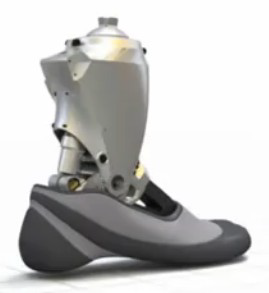
\includegraphics[width=.8\textwidth]{images/prot_01}
}%figues de la page de garde

\def\xxpied{%
DS 3 -- Tracé de l'abaque de temps de réponse réduit}


\setcounter{secnumdepth}{5}
%---------------------------------------------------------------------------


\begin{document}

%\chapterimage{png/Fond_Cin}
\pagestyle{empty}


%%%%%%%% PAGE DE GARDE COURS
\ifcours
\begin{tikzpicture}[remember picture,overlay]
\node at (current page.north west)
{\begin{tikzpicture}[remember picture,overlay]
\node[anchor=north west,inner sep=0pt] at (0,0) {\includegraphics[width=\paperwidth]{\thechapterimage}};
\draw[anchor=west] (-2cm,-8cm) node [line width=2pt,rounded corners=15pt,draw=ocre,fill=white,fill opacity=0.6,inner sep=40pt]{\strut\makebox[22cm]{}};
\draw[anchor=west] (1cm,-8cm) node {\huge\sffamily\bfseries\color{black} %
\begin{minipage}{1cm}
\rotatebox{90}{\LARGE\sffamily\textsc{\color{ocre}\textbf{\xxnumpartie}}}
\end{minipage} \hfill
\begin{minipage}[c]{14cm}
\begin{titrepartie}
\begin{flushright}
\renewcommand{\baselinestretch}{1.1} 
\Large\sffamily\textsc{\textbf{\xxpartie}}
\renewcommand{\baselinestretch}{1} 
\end{flushright}
\end{titrepartie}
\end{minipage} \hfill
\begin{minipage}[c]{3.5cm}
{\large\sffamily\textsc{\textbf{\color{ocre} \discipline}}}
\end{minipage} 
 };
\end{tikzpicture}};
\end{tikzpicture}


\begin{tikzpicture}[overlay]
\node[shape=rectangle, 
      rounded corners = .25 cm,
	  draw= ocre,
	  line width=2pt, 
	  fill = ocre!10,
	  minimum width  = 2.5cm,
	  minimum height = 3cm,] at (18cm,0) {};
\node at (17.7cm,0) {\rotatebox{90}{\textbf{\Large\color{ocre}{\classe}}}};
%{};
\end{tikzpicture}

\vspace{3.5cm}

\begin{tikzpicture}[remember picture,overlay]
\draw[anchor=west] (-2cm,-6cm) node {\huge\sffamily\bfseries\color{black} %
\begin{minipage}{2cm}
\begin{center}
\LARGE\sffamily\textsc{\color{ocre}\textbf{\xxactivite}}
\end{center}
\end{minipage} \hfill
\begin{minipage}[c]{15cm}
\begin{titrechapitre}
\renewcommand{\baselinestretch}{1.1} 
\Large\sffamily\textsc{\textbf{\xxnumchapitre}}

\Large\sffamily\textsc{\textbf{\xxchapitre}}
\vspace{.5cm}

\renewcommand{\baselinestretch}{1} 
\normalsize\normalfont
\xxcompetences
\end{titrechapitre}
\end{minipage}  };
\end{tikzpicture}
\vfill

\begin{flushright}
\begin{minipage}[c]{.3\linewidth}
\begin{center}
\xxfigures
\end{center}
\end{minipage}\hfill
\begin{minipage}[c]{.6\linewidth}
\startcontents
\printcontents{}{1}{}
\end{minipage}
\end{flushright}

\begin{tikzpicture}[remember picture,overlay]
\draw[anchor=west] (4.5cm,-.7cm) node {
\begin{minipage}[c]{.2\linewidth}
\begin{flushright}

\includegraphics[width=2cm]{png/logoCC}
\end{flushright}
\end{minipage}
\begin{minipage}[c]{.2\linewidth}
\textsl{\xxauteur} \\
\textsl{\classe}
\end{minipage}
 };
\end{tikzpicture}
\newpage
\pagestyle{fancy}

\newpage
\pagestyle{fancy}

\else
\fi


%%%%%%%% PAGE DE GARDE TD
\iftd
%\begin{tikzpicture}[remember picture,overlay]
%\node at (current page.north west)
%{\begin{tikzpicture}[remember picture,overlay]
%\draw[anchor=west] (-2cm,-3.25cm) node [line width=2pt,rounded corners=15pt,draw=ocre,fill=white,fill opacity=0.6,inner sep=40pt]{\strut\makebox[22cm]{}};
%\draw[anchor=west] (1cm,-3.25cm) node {\huge\sffamily\bfseries\color{black} %
%\begin{minipage}{1cm}
%\rotatebox{90}{\LARGE\sffamily\textsc{\color{ocre}\textbf{\xxnumpartie}}}
%\end{minipage} \hfill
%\begin{minipage}[c]{13.5cm}
%\begin{titrepartie}
%\begin{flushright}
%\renewcommand{\baselinestretch}{1.1} 
%\Large\sffamily\textsc{\textbf{\xxpartie}}
%\renewcommand{\baselinestretch}{1} 
%\end{flushright}
%\end{titrepartie}
%\end{minipage} \hfill
%\begin{minipage}[c]{3.5cm}
%{\large\sffamily\textsc{\textbf{\color{ocre} \discipline}}}
%\end{minipage} 
% };
%\end{tikzpicture}};
%\end{tikzpicture}

%%%%%%%%%% PAGE DE GARDE TD %%%%%%%%%%%%%%%
%\begin{tikzpicture}[overlay]
%\node[shape=rectangle, 
%      rounded corners = .25 cm,
%	  draw= ocre,
%	  line width=2pt, 
%	  fill = ocre!10,
%	  minimum width  = 2.5cm,
%	  minimum height = 2.5cm,] at (18.5cm,0) {};
%\node at (17.7cm,0) {\rotatebox{90}{\textbf{\Large\color{ocre}{\classe}}}};
%%{};
%\end{tikzpicture}

% PARTIE ET CHAPITRE
%\begin{tikzpicture}[remember picture,overlay]
%\draw[anchor=west] (-1cm,-2.1cm) node {\large\sffamily\bfseries\color{black} %
%\begin{minipage}[c]{15cm}
%\begin{flushleft}
%\xxnumchapitre \\
%\xxchapitre
%\end{flushleft}
%\end{minipage}  };
%\end{tikzpicture}

% Bandeau titre exo
\begin{tikzpicture}[remember picture,overlay]
\draw[anchor=west] (-2cm,-4cm) node {\huge\sffamily\bfseries\color{black} %
\begin{minipage}{5cm}
\begin{center}
\LARGE\sffamily\color{ocre}\textbf{\textsc{\xxactivite}}

\begin{center}
\xxfigures
\end{center}

\end{center}
\end{minipage} \hfill
\begin{minipage}[c]{12cm}
\begin{titrechapitre}
\renewcommand{\baselinestretch}{1.1} 
\large\sffamily\textbf{\textsc{\xxtitreexo}}

\small\sffamily{\textbf{\textit{\color{black!70}\xxsourceexo}}}
\vspace{.5cm}

\renewcommand{\baselinestretch}{1} 
\normalsize\normalfont
\xxcompetences
\end{titrechapitre}
\end{minipage}  };
\end{tikzpicture}
\else
\fi


%%%%%%%% PAGE DE GARDE FICHE
\iffiche
\begin{tikzpicture}[remember picture,overlay]
\node at (current page.north west)
{\begin{tikzpicture}[remember picture,overlay]
\draw[anchor=west] (-2cm,-3.25cm) node [line width=2pt,rounded corners=15pt,draw=ocre,fill=white,fill opacity=0.6,inner sep=40pt]{\strut\makebox[22cm]{}};
\draw[anchor=west] (1cm,-3.25cm) node {\huge\sffamily\bfseries\color{black} %
\begin{minipage}{1cm}
\rotatebox{90}{\LARGE\sffamily\textsc{\color{ocre}\textbf{\xxnumpartie}}}
\end{minipage} \hfill
\begin{minipage}[c]{14cm}
\begin{titrepartie}
\begin{flushright}
\renewcommand{\baselinestretch}{1.1} 
\large\sffamily\textsc{\textbf{\xxpartie} \\} 

\vspace{.2cm}

\normalsize\sffamily\textsc{\textbf{\xxnumchapitre -- \xxchapitre}}
\renewcommand{\baselinestretch}{1} 
\end{flushright}
\end{titrepartie}
\end{minipage} \hfill
\begin{minipage}[c]{3.5cm}
{\large\sffamily\textsc{\textbf{\color{ocre} \discipline}}}
\end{minipage} 
 };
\end{tikzpicture}};
\end{tikzpicture}


\begin{tikzpicture}[overlay]
\node[shape=rectangle, 
      rounded corners = .25 cm,
	  draw= ocre,
	  line width=2pt, 
	  fill = ocre!10,
	  minimum width  = 2.5cm,
	  minimum height = 2.5cm,] at (18.5cm,0.5cm) {};
%	  minimum height = 2.5cm,] at (18.5cm,0cm) {};
\node at (17.7cm,0.5) {\rotatebox{90}{\textsf{\textbf{\large\color{ocre}{\classe}}}}};
%{};
\end{tikzpicture}

\else
\fi



\vspace{2cm}
\pagestyle{fancy}
\thispagestyle{plain}

\section{Mise en situation}


L'équation différentielle d'un système du second ordre peut se mettre sous la forme :

\vspace{.25cm}

\begin{minipage}[c]{.48\linewidth}
$$
s(t)
+\dfrac{2\xi}{\omega_0}\cdot \dfrac{\text{d}s(t)}{\text{d}t}
+\dfrac{1}{\omega_0^2}\cdot \dfrac{\text{d}^2s(t)}{\text{d}t^2}
= K\cdot e(t)
$$
\end{minipage}\hfill
\begin{minipage}[c]{.48\linewidth}
en notant :
\begin{itemize}
\item $K$ : le gain statique;
\item $\xi$ : le coefficient d'amortissement;
\item $e(t)$ et $s(t)$ : l'entrée et la sortie du système. 
\end{itemize}
\end{minipage}


\begin{minipage}[c]{.48\linewidth}
\begin{obj}
L'objectif de ces travaux est de construire le programme permettant de tracer l'abaque du temps de réponse réduit utilisé en asservissement pour connaître le temps de réponse à 5\% des systèmes d'ordre 2. 
\end{obj}
\end{minipage}\hfill
\begin{minipage}[c]{.5\linewidth}
\begin{center}
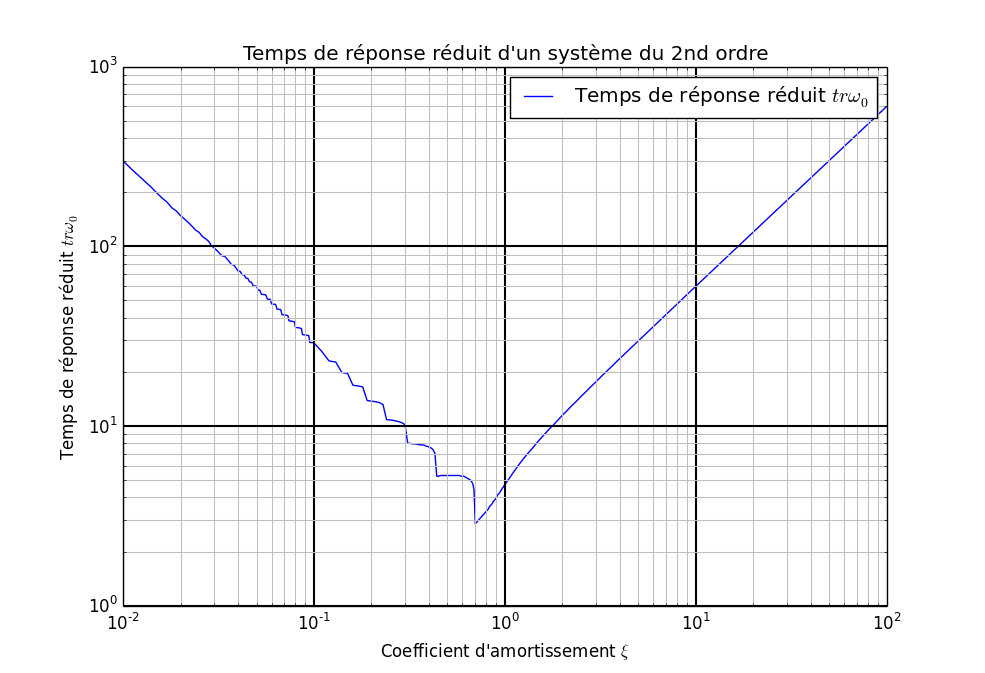
\includegraphics[width=.95\textwidth]{images/figure_1}
\end{center}
\end{minipage}

\section{Résolution de l'équation différentielle}

On cherche à résoudre $
s(t)
+\dfrac{2\xi}{\omega_0}\cdot \dfrac{\text{d}s(t)}{\text{d}t}
+\dfrac{1}{\omega_0^2}\cdot \dfrac{\text{d}^2s(t)}{\text{d}t^2}
= K\cdot e(t)
$.
On pose : 
$
\left\{ 
\begin{array}{l}
y_1(t)=s(t) \\
y_2(t)=\dfrac{\text{d}s(t)}{\text{d} t}
\end{array}
\right.
$.

\subparagraph{}
\textit{Donner la solution \textbf{numérique} de l'équation différentielle du second ordre en utilisant le changement de variable proposé et le schéma d'Euler explicite. On notera $h$ le pas du schéma.}


\ifprof
\begin{corrige}
D'après le schéma d'Euler explicite, on a $s_{k+1}=s_{k}+hy_{1,k}$. 
\end{corrige}
\else
\fi


\subparagraph{}
\textit{Donner la solution \textbf{numérique} de l'équation différentielle $y_2(t)=\dfrac{\text{d}s(t)}{\text{d} t}$ en utilisant un schéma d'Euler explicite. Vous mettrez la solution sous la forme
$ \left\{ 
\begin{array}{l}
y_{1,k+1}=y_{1,k}+h \Phi_{1,k} \\
y_{2,k+1}=y_{2,k}+h \Phi_{2,k} \\
\end{array}
\right.
$ avec $\Phi_{1,k}$ et $\Phi_{2,k}$ deux fonctions à expliciter.}

\ifprof
\begin{corrige}
En appliquant le changement de variable à l'équation différentielle, on a :
$$
\left\{ 
\begin{array}{l}
y_2(t)=\dfrac{\text{d}y_1(t)}{\text{d}t} \\
y_1(t)
+\dfrac{2\xi}{\omega_0}\cdot y_2(t)
+\dfrac{1}{\omega_0^2}\cdot \dfrac{\text{d}y_2(t)}{\text{d}t}
= K\cdot e(t) \\
\end{array}
\right.
\Leftrightarrow 
\left\{ 
\begin{array}{l}
y_2(t)=\dfrac{\text{d}y_1(t)}{\text{d}t} \\
y_1(t)
+\dfrac{2\xi}{\omega_0}\cdot y_2(t)
+\dfrac{1}{\omega_0^2}\cdot \dfrac{\text{d}y_2(t)}{\text{d}t}
= K\cdot e(t) \\
\end{array}
\right.
$$

En utilisant la formulation de Cauchy, on a :
$$
\left\{ 
\begin{array}{l}
\Phi_1(t,y_1(t),y_2(t))=y_2(t)\\
\Phi_2(t,y_1(t),y_2(t))=K\omega_0^2\cdot e(t) - 2\xi \omega_0  y_2(t) -\omega_0^2y_1(t)\\
\end{array}
\right.
.
$$

En utilisant le schéma d'Euler explicite, on a donc : 

$$
\left\{ 
\begin{array}{l}
y_{1,k+1}=y_{1,k}+h \Phi_1(t_k,y_{1,k},y_{2,k}) \\
y_{2,k+1}=y_{2,k}+h \Phi_2(t_k,y_{1,k},y_{2,k}) \\
\end{array}
\right.
\Rightarrow
\left\{ 
\begin{array}{l}
y_{1,k+1}=y_{1,k}+h y_{2,k} \\
y_{2,k+1}=y_{2,k}+h \left( K\omega_0^2\cdot e_k - 2\xi \omega_0  y_{2,k} -\omega_0^2y_{1,k}\right) \\
\end{array}
\right.
.
$$
\end{corrige}
\else
\fi

Les variables $K$, $\omega_0$, $\xi$, $h$ sont données. On considère que $s(0)=0$ et $s'(0)=0$. On considère que les fonctions $\Phi_1(k)$ et $\Phi_2(k)$ ont été implémentées et peuvent être évaluées en utilisant les fonctions Python \texttt{phi\_1} et \texttt{phi\_2} . On note $T$ le temps de simulation.


\subparagraph{}
\textit{Donner en Python la suite d'instructions permettant de disposer des listes \texttt{les\_y1} et \texttt{les\_y2}.}


\subparagraph{}
\textit{Donner en Python la suite d'instructions permettant de tracer la réponse du système en fonction du temps.}

\section{Recherche du temps de réponse à 5\%}

\subparagraph{}
\textit{Pour $K=1$ et pour une entrée de type échelon, tracer l'allure de la réponse temporelle pour $\xi<0,7$ et pour $\xi>1$. Pour chacune des courbes deux courbes, afficher le temps de réponse à 5\%.}

\vspace{.5cm}

Pour un système du second ordre de gain $K=1$ sollicité par un échelon, il est nécessaire de résoudre l'équation $s(t)=0,95$ et $s(t)=1,05$ pour déterminer le temps de réponse à 5\%.

\subparagraph{}
\textit{En utilisant des schémas (un schéma par méthode), expliquer la méthode de résolution de l'équation en utilisant la méthode de Newton et en utilisant une méthode par dichotomie.}


\subparagraph{}
\textit{Donner l'algorithme de la méthode de Newton.}


\subparagraph{}
\textit{Dans notre cas, quelle méthode semble la plus appropriée ? Quel(s) problème(s) peut-on rencontrer ? Comment l'(es) éviter ? }



\subparagraph{}
\textit{Proposer une méthode pour déterminer le temps de réponse à 5\%. }


\section{Tracé de l'abaque de temps de réponse à 5 \%}


\ifprof
\else
On reprend l'équation différentielle présentée précédemment. On suppose que toutes les conditions initiales sont nulles. Pour une entrée unitaire de type échelon unitaire $e(t)=1$, $K=1$ et $t\geq0$ on montre que : 
\begin{itemize}
\item si $\xi <1$, le régime est pseudo périodique et :
$
s(t)=1-\dfrac{e^{-\xi\omega_0 t}}{\sqrt{1-\xi^2}}\sin\left(  \omega_0 t\sqrt{1-\xi^2}+\arcsin \sqrt{1-\xi^2} \right)
$;
\item si $\xi=1$, le régime est critique et : 
$
s(t)=1-\left(1+\omega_0 t \right)e^{-\omega_0 t} 
$;
\item si $\xi>1$, le régime est apériodique et : 
$
s(t)=1
+\dfrac{e^{- \omega_0 t\left( \xi + \sqrt{\xi^2-1}\right)}}{2\left(\xi\sqrt{\xi^2-1}+\xi^2-1 \right)}
-\dfrac{e^{- \omega_0 t \left( \xi - \sqrt{\xi^2-1}\right)}}{2\left(\xi\sqrt{\xi^2-1}-\xi^2+1 \right)}
$.
\end{itemize} 


\textbf{Dans la suite, on considèrera que $s$ est une fonction du temps réduit $t\cdot\omega_0$ que l'on notera $t\omega_0$ ou \texttt{tom0}. On notera indifféremment le coefficient d'amortissement $z$ ou $\xi$.}



\fi

\ifprof
\else
On dispose des fonctions Python \texttt{f\_pseudo}, \texttt{f\_critique} et \texttt{f\_aperiodique} permettant d'évaluer la fonction pour $s$ pour un couple $(t\omega_0,\xi)$.
\fi




\subparagraph{} \textit{Donner, en Python, le contenu de la fonction \textsf{f\_s} permettant de définir la fonction $(t\omega_0,\xi) \rightarrow s(t\omega_0\xi)$ dans le cas où $\xi\in \mathbb{R}_+^*$. On donne ci-dessous les spécifications de la fonction.}
\ifprof
\else
\begin{py}
\begin{python}
def f_s(tom0,z):
    """
    Fonction permettant de calculer la réponse indicielle d'un système du second ordre. 
    Entrées : 
        * tom0, flt : temps de réponse réduit
        * z, flt : coefficient d'amortissement
    Sortie : 
        * s(tom0,z), flt
    """
\end{python}
\end{py}
\fi

\ifprof
\begin{corrige}
\begin{py}
\begin{python}
def f_s(tom0,z) :
    """
    Fonction permettant de calculer la réponse indicielle d'un système du second ordre. 
    Entrées : 
        * tom0, flt : temps de réponse réduit
        * z, flt : coefficient d'amortissement
    Sortie : 
        * s(tom0,z), flt
    """
    if z<0 :
        return None
    elif z<1 :
        return f2_pseudo(tom0,z)
    elif z==1:
        return f2_critique(tom0)
    else : 
        return f2_aperiodique(tom0,z)
\end{python}
\end{py}
\end{corrige}
\else

%\begin{tabular}{|p{.95\textwidth}|}
%\hline
%$$\quad$$
%\vspace{4cm}
%$$\quad$$ \\
%\hline
%\end{tabular}
\fi

\ifprof
\else

%\newpage 
%
%La fonction \texttt{trace\_s} donnée ci-dessous permet de tracer $s(t\omega_0,\xi)$ pour $t\omega_0 \in [0,10]$ par pas de 1 et pour une valeur de $\xi$ déterminée. Les deux appels successifs de la fonction \texttt{trace\_s} permettent de réaliser le tracer les 2 courbes ci-dessous.
%
%
%\begin{minipage}[c]{.48\linewidth}
%\begin{py}
%\begin{python}
%# Définition de la fonction trace
%def trace_s(z):
%    x = []
%    y = []
%    for i in range(11):
%        t = i
%        x.append(t)
%        y.append(f_s(t,z))
%    plot(x,y)
%# Appels de la fonction trace
%trace_s(0.4)
%trace_s(0.7)
%
%\end{python}
%\end{py}
%\end{minipage} \hfill
%\begin{minipage}[c]{.48\linewidth}
%\begin{center}
%%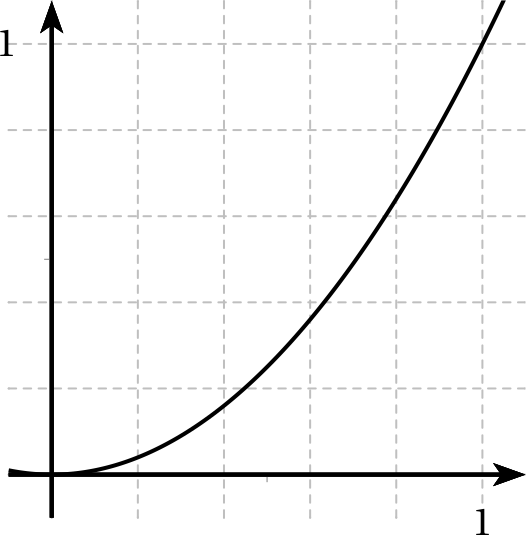
\includegraphics[width=\textwidth]{images/courbe}
%\end{center}
%\end{minipage}
%\fi

%
%\subparagraph{}
%\textit{Expliquer l'objectif des lignes 2 à 9.}
%
%\ifprof
%\begin{corrige}
%\begin{itemize}
%\item La ligne 2 permet de définir la fonction.
%\item Les lignes 3 et 4 permettent d'initialiser deux listes.
%\item Les lignes 5 à 8 vont permettre de créer deux listes de 11 éléments. Ainsi la liste x contiendra le temps réduit de 0 à 10 et la liste y contiendra les valeurs de s(x) pour chacune de ces 11 valeurs. 
%\end{itemize}
%\end{corrige}
%\else
%\begin{tabular}{|p{.95\textwidth}|}
%\hline
%$$\quad$$
%\vspace{3cm}
%$$\quad$$ \\
%\hline
%\end{tabular}
%\ifprof
%\else
%
%\vspace{1cm}
%
%\fi
%
%
%On observe que la courbe tracée n'est pas lissée. Pour avoir un meilleur rendu, il est nécessaire d'évaluer la fonction en davantage de points. 
%\fi
%
%\subparagraph{}
%\textit{Modifier les lignes 5 et 6 pour que la courbe tracée soit réalisée en 1000 points sur un intervalle de $t \omega_0$ variant de 0 à 10. }
%
%\ifprof
%\begin{corrige}
%\begin{py}
%\begin{python}
%def trace_s(z):
%    x = []
%    y = []
%    n = 1000
%    for i in range(n+1):
%        t = 10*i/n
%        x.append(t)
%        y.append(f_s(t,z))
%    plot(x,y)
%\end{python}
%\end{py}
%\end{corrige}
%\else
%
%\begin{tabular}{|p{.95\textwidth}|}
%\hline
%$$\quad$$
%\vspace{2cm}
%$$\quad$$ \\
%\hline
%\end{tabular}
%\newpage
%\fi

%\subsection*{Tracé de l'abaque}

On note $t_r$  le temps de réponse à 5\%. L'abaque du temps de réponse permet de tracer le produit $t_r\omega_0$ en fonction du coefficient d'amortissement $\xi$.

\subparagraph{}
\textit{Quelle est la valeur finale prise par $s(t)$ ?} 
\ifprof
\begin{corrige}
La valeur finale est 1. 
\end{corrige}
\else


%\begin{tabular}{|p{.95\textwidth}|}
%\hline
%$$\quad$$ \\
%\hline
%\end{tabular}

\fi


\subparagraph{}
\textit{Écrire en Python la fonction \textsf{\textbf{is\_in\_strip}} ayant les spécifications suivantes : } 
\ifprof
\else

\begin{py}
\begin{python}
def is_in_strip(x):
    """
    Fonction permettant de savoir si une valeur est dans la bande des + ou - 5% de la valeur finale.
    Entrée : 
        x, flt : réel
    Sortie : 
        True si la valeur est dans la bande à + ou - 5%
        False si la valeur n'est pas dans la bande à + ou - 5%
    """
\end{python}
\end{py}
\fi

\ifprof
\begin{corrige}
\begin{py}
\begin{python}
def is_in_strip(x):
    """
    Fonction permettant de savoir si une valeur est dans la bande des + ou - 5% de la valeur finale.
    Entrée : 
        x, flt : réel
    Sortie : 
        True si la valeur est dans la bande à + ou - 5%
        False si la valeur n'est pas dans la bande à + ou - 5%
    """
    if x>.95 and x<1.05:
        return True
    else:
        return False
\end{python}
\end{py}
\end{corrige}
\else
%
%
%\begin{tabular}{|p{.95\textwidth}|}
%\hline
%$$\quad$$
%\vspace{2cm}
%$$\quad$$ \\
%\hline
%\end{tabular}
\fi

\ifprof
\else
\vspace{1cm}

On donne la fonction suivante permettant de connaître le temps de réponse réduit à partir duquel la réponse indicielle d'un système est dans la bande à plus ou moins 5\% pour un coefficient d'amortissement particulier.

\begin{py}
\begin{python}
def calcul_tom0(z,tom0=500):
    """
    Recherche du temps de réponse à 5%
    Entrées : 
       * z, flt : coefficient d'amortissement
       * tom0 (flt, optionnel) : si non précisé, on calcule le temps de réponse en partant de tom0 = 500
    Sortie : 
       * tom0 (flt) : temps de réponse à 5%
    """
    pas_tom0=0.05
    x = f_s(tom0,z) 
    if z<0.7:
        while is_in_strip(x) :
            tom0  = tom0 - pas_tom0
            x = f_s(tom0,z)
        tom0=tom0+pas_tom0
    else :
        while not is_in_strip(x) :
            tom0  = tom0 + pas_tom0 
            x = f_s(tom0,z)
        tom0=tom0-pas_tom0
    return tom0
\end{python}
\end{py}


\fi



\subparagraph{}
\textit{Expliquer le mode de recherche du temps de réponse à 5\% dans le cas où $z<0,7$ puis dans le cas où $z\geq 0,7$. Pourquoi distingue-t-on ces 2 cas ? On pourra s'aider de l'abaque donné sur la première page.}

\ifprof
\else
%\begin{rem}
%On pourra remarquer que dans un cas, la recherche se fait << en avançant >> et dans le second cas << en reculant >>. 
%\end{rem}

%
%\begin{tabular}{|p{.95\textwidth}|}
%\hline
%$$\quad$$
%\vspace{1cm}
%$$\quad$$ \\
%\hline
%\end{tabular}
%
%\vspace{1cm}

\fi

\ifprof
\begin{corrige}
Pour déterminer le temps de réponse à 5\%, on cherche le dernier temps pour lequel, le signal est dans la bande à plus ou moins 5\%. En régime permanent, le signal est dans la bande. En << remontant le temps >> la première valeur hors de la bande correspond donc au temps de réponse recherché. 

Lorsque $\xi<0,7$, le système est oscillant, et le temps de réponse est mesuré lorsque les oscillations deviennent <<petites>>. Il est donc préférable de partir de la fin.

Lorsque $\xi>0,7$, on sait que dès lors que le signal entre dans la bande, il n'en sortira plus. Il est donc plus rapide de commencer par le début. 

\end{corrige}
\else
\fi

\ifprof
\else

\vspace{.5cm}

L'algorithme suivant permet de créer les listes \textsf{xx} et \textsf{yy} permettant de tracer l'abaque du temps de réponse réduit en fonction du coefficient d'amortissement. 

\begin{py}
\begin{python}
xx,yy = [],[]
n = 1000
z = 0.01
tom0 = 500
pasz = 0.01
while z<=100:
    if z<0.7:
        tom0=calcul_tom0(z,tom0)
    else :
        tom0=calcul_tom0(z,0)  
    if z<0.1:
        pasz = 0.001
    elif z<1:
        pasz = 0.01
    elif z<10:
        pasz = 0.1
    else :
        pasz = 1    
    xx.append(z)
    yy.append(tom0)
    z=z+pasz
\end{python}
\end{py}

%\newpage
\fi


 

\subparagraph{}
\textit{
\begin{enumerate}
\item Donner l'intervalle de variation de \textsf{z} pour le tracé demandé.
\item Donner le pas de \textsf{z} sur chacun des intervalles.
\item Pourquoi ne pas conserver le même pas sur chacun de ces intervalles ?
\item En vous aidant du tracé de l'abaque, expliquer pourquoi \textsf{tom0} est calculé différemment suivant la valeur de \textsf{z} ? Expliquer le choix des arguments de la fonction \textsf{calcul\_tom0} dans chacun des cas. 
\end{enumerate}}
\ifprof
\begin{corrige}
\begin{enumerate}
\item $z$ variera de 0,01 à 100.
\item On a : 
\begin{itemize}
\item si $0,01<z<0,1$ : $pasz = 0,001$;
\item si $0,1<z<1$ : $pasz = 0,01$;
\item si $1<z<10$ : $pasz = 0,1$;
\item si $10<z<100$ : $pasz = 1$.
\end{itemize}
\item La courbe est tracée en diagramme log-log. On adopte donc un pas différent par décade. 
\item Lorsque $\xi<0.7$, $tom0$ décroit lorsque $z$ croît. Pour trouver plus rapidement $tom0$ on peut donc utiliser la valeur prise précédemment (dans ce cas, la recherche de tom0 dans la fonction \textsf{calcul\_tom0} se fait à rebours). A l'inverse, lorsque $\xi>0.7$, $tom0$ croit lorsque $z$ croît. On choisit dans ce cas, de partir à chaque fois de 0 (en modifiant le code, il serait possible de partir du $tom0$ calculé précédemment, mais il faudrait réfléchir à la gestion de la bascule de $\xi<0,7$ à $\xi>0,7$).
\end{enumerate}
\end{corrige}
\else

%
%\begin{tabular}{|p{.95\textwidth}|}
%\hline
%$$\quad$$
%\vspace{6cm}
%$$\quad$$ \\
%\hline
%\end{tabular}

\fi

\subparagraph{}
\textit{On souhaite stocker les données des listes \textsf{xx} et \textsf{yy} dans un fichier texte encodé en ASCII. Chacun des nombres doit être stocké sur 17 caractères. Indiquer la taille du fichier ainsi créé.}
\ifprof
\begin{corrige}
90 valeurs sont calculées pour chaque intervalles de $z$. $xx$ et $yy$ ont donc une taille de 360 éléments. 
En prenant en compte les 34 caractères, l'espace et le retour à la ligne (2 caractères), une ligne a donc une taille de 37 octets. Le fichier sera donc d'approximativement de 13 320 octets.
\end{corrige}
\else

%\begin{tabular}{|p{.95\textwidth}|}
%\hline
%$$\quad$$
%\vspace{2cm}
%$$\quad$$ \\
%\hline
%\end{tabular}

\fi
\ifprof
\else
%
%
%\begin{py}
%\begin{python}
%import matplotlib.pyplot as plt
%import numpy as np
%
%plt.plot(xx,yy,label="Temps de réponse réduit $tr \\omega_0$")
%plt.xlabel("Coefficient d'amortissement $\\xi$")
%plt.ylabel("Temps de réponse réduit $tr \\omega_0$")
%plt.title("Temps de réponse réduit d'un système du 2nd ordre")
%plt.legend()
%plt.loglog()
%plt.grid(which="major",axis="x",linewidth=1.5, linestyle='-')
%plt.grid(which="major",axis="y",linewidth=1.5, linestyle='-')
%plt.grid(which="minor",axis="x",linewidth=0.75, linestyle='-', color='0.75')
%plt.grid(which="minor",axis="y",linewidth=0.75, linestyle='-', color='0.75')
%\end{python}
%\end{py}
%%
%%\begin{figure}[!ht]
%%\begin{center}
%%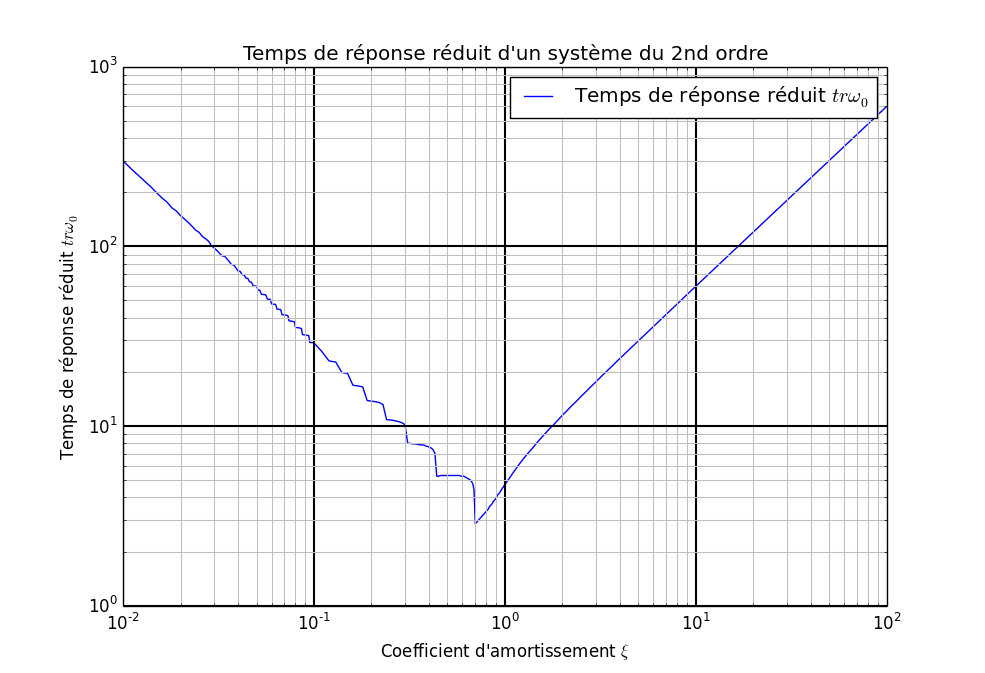
\includegraphics[width=.8\linewidth]{images/figure_1}
%%
%%Abaque du temps de réponse réduit pour un système du second ordre \label{ref_aba}
%%\end{center}
%%\end{figure}
\fi

\section*{Question supplémentaire}

\subparagraph{}
\textit{En utilisant la méthode des trapèzes, calculer l'intégrale de $s(t)$ pour un intervalle de $T$ secondes, avec un pas de temps $h$.}

\end{document}
